\documentclass[10pt]{article} % Font size - 10pt, 11pt or 12pt

\usepackage[hmargin=1.25cm, vmargin=1.5cm]{geometry} % Document margins

\usepackage{marvosym} % Required for symbols in the colored box
\usepackage{ifsym} % Required for symbols in the colored box

\usepackage[usenames,dvipsnames]{xcolor} % Allows the definition of hex colors

% Fonts and tweaks for XeLaTeX
\usepackage{fontspec,xltxtra,xunicode}
\defaultfontfeatures{Mapping=tex-text}
%\setmonofont[Scale=MatchLowercase]{Andale Mono}

% Colors for links, text and headings
\usepackage{hyperref}
\definecolor{linkcolor}{HTML}{506266} % Blue-gray color for links
\definecolor{shade}{HTML}{F5DD9D} % Peach color for the contact information box
\definecolor{text1}{HTML}{2b2b2b} % Main document font color, off-black
\definecolor{headings}{HTML}{701112} % Dark red color for headings
% Other color palettes: shade=B9D7D9 and linkcolor=A40000; shade=D4D7FE and linkcolor=FF0080

\hypersetup{colorlinks,breaklinks, urlcolor=linkcolor, linkcolor=linkcolor} % Set up links and colors

\usepackage{fancyhdr}
\usepackage{amsmath}
\usepackage{amssymb}
\pagestyle{fancy}
\fancyhf{}
% Headers and footers can be added with the \lhead{} \rhead{} \lfoot{} \rfoot{} commands
% Example footer:
%\rfoot{\color{headings} {\sffamily Last update: \today}. Typeset with Xe\LaTeX}

\renewcommand{\headrulewidth}{0pt} % Get rid of the default rule in the header

\usepackage{titlesec} % Allows creating custom \section's

% Format of the section titles
\titleformat{\section}{\color{headings}
\scshape\Large\raggedright}{}{0em}{}[\color{black}\titlerule]

\title{Solid State Assignment One}
\author{Elliott Capek}
\titlespacing{\section}{0pt}{0pt}{5pt} % Spacing around titles

\begin{document}

\maketitle{}

\section{Problem 1: D functions as linear combinations}
For each of the five d-orbitals wavefunctions, create a 3D plot of the angular wave and express
the angular wave as a linear combination of spherical harmonics, like so:

\begin{align*}
  d_{x^2-y^2} &= a_{00}Y_{00} + a_{1-1}Y_{1-1} + a_{10}Y_{10} + a_{11}Y_{11} + a_{20}Y_{20} + ...\\
\end{align*}

First, we use Mathematica to plot the wave functions:

\begin{figure}[h!]
  \centering
  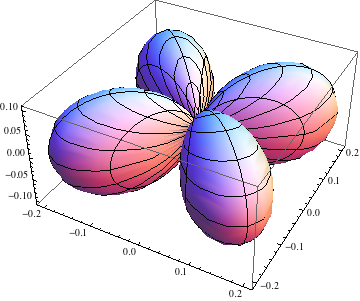
\includegraphics[width=0.2\textwidth]{../figures/dxy.png}
  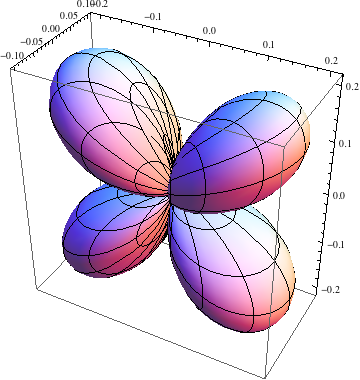
\includegraphics[width=0.2\textwidth]{../figures/dyz.png}
  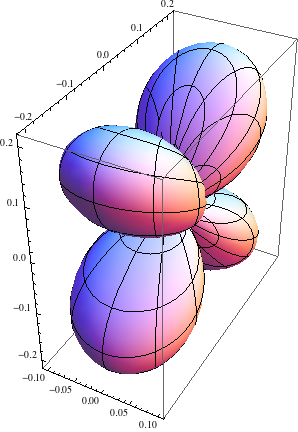
\includegraphics[width=0.2\textwidth]{../figures/dzx.png}
  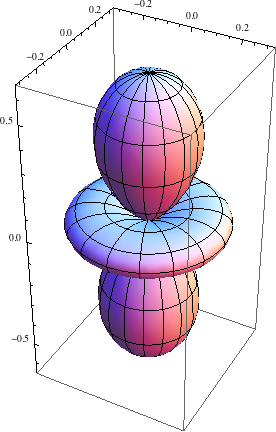
\includegraphics[width=0.2\textwidth]{../figures/dz2.png}
  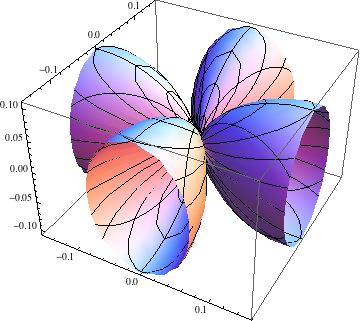
\includegraphics[width=0.2\textwidth]{../figures/dx2y2.png}
  \caption{From first to last: $d_{xy}$, $d_{yz}$, $d_{zx}$, $d_{z^2}$ and $d_{x^2-y^2}$, all on the same XY plane}
  \label{fig:dxy}
\end{figure}

We then convert the Cartesian d wavefunctions from Stross Eq 1.22 into spherical
coordinates, so we can more easily see which spherical harmonics they are made
up of.\\

\begin{align*}
  x &= r\cos(\phi)\sin(\theta)\\
  y &= r\sin(\phi)\sin(\theta)\\
  z &= r\cos(\theta)\\
\end{align*}

\begin{align*}
  d_{xy} &= \left(\frac{15}{4\pi}\right)^{1/2}\frac{xy}{r^2}
  = \left(\frac{15}{4\pi}\right)^{1/2}\cos(\phi)\sin(\phi)\sin^2(\theta)\\
  d_{yz} &= \left(\frac{15}{4\pi}\right)^{1/2}\frac{yz}{r^2}
  = \left(\frac{15}{4\pi}\right)^{1/2}\sin(\phi)\sin(\theta)\cos(\theta)\\
  d_{zx} &= \left(\frac{15}{4\pi}\right)^{1/2}\frac{zx}{r^2}
  = \left(\frac{15}{4\pi}\right)^{1/2}\cos(\phi)\sin(\theta)\cos(\theta)\\
  d_{z^2} &= \left(\frac{15}{4\pi}\right)^{1/2}
  \left(\frac{3z^2-r^2}{2\sqrt{3}r^2}\right)
  = \left(\frac{15}{4\pi}\right)^{1/2}
  \left(\frac{3\cos^2(\theta)-1}{2\sqrt{3}}\right)\\
  d_{x^2-y^2} &= \left(\frac{15}{4\pi}\right)^{1/2}
  \left(\frac{x^2-y^2}{2r^2}\right)
  = \left(\frac{15}{4\pi}\right)^{1/2}
  \frac{\cos^2(\phi)\sin^2(\theta)-\sin^2(\phi)\sin^2(\theta)}{2}\\
\end{align*}

We then write these real-basis functions as linear combinations of spherical harmonics:

\begin{align*}
  d_{xy} &= \frac{i}{\sqrt{2}}\left(Y_{2-2} - Y_{22}\right)
  = \frac{i}{\sqrt{2}}\left(\frac{15}{32\pi}\right)^{1/2}
  \sin^2\theta\left(e^{2i\phi}-e^{-2i\phi}\right)
  = \left(\frac{15}{4\pi}\right)^{1/2}\sin^2\theta\sin\theta\cos\theta\\
  d_{yz} &= \frac{i}{\sqrt{2}}\left(Y_{2-1}+Y_{21}\right)\\
  d_{zx} &= \frac{1}{\sqrt{2}}\left(Y_{2-1}-Y_{21}\right)\\
  d_{z^2} &= Y_{20}\\
  d_{x^2-y^2} &= \frac{1}{\sqrt{2}}\left(Y_{22} + Y_{2-2}\right)\\
\end{align*}

\section{2: Matrix representation of operators}
First, we write the matrix representation of the two angular momentum operators. Here
the spherical harmonics for $\ell=2$ are orthogonal unit vectors, so $Y_{2-2}=(1 0 0 0 0)^T$, etc...\\

\begin{align*}
  L^2 =
  6\hbar^2\begin{pmatrix}
    1 & 0 & 0 & 0 & 0\\
    0 & 1 & 0 & 0 & 0\\
    0 & 0 & 1 & 0 & 0\\
    0 & 0 & 0 & 1 & 0\\
    0 & 0 & 0 & 0 & 1\\
  \end{pmatrix}&
  \hspace{2cm}
  L_z =
  \hbar\begin{pmatrix}
    -2 & 0 & 0 & 0 & 0\\
    0 & -1 & 0 & 0 & 0\\
    0 & 0 & 0 & 0 & 0\\
    0 & 0 & 0 & 1 & 0\\
    0 & 0 & 0 & 0 & 2\\
  \end{pmatrix}
\end{align*}

Now we compute the same matrices for the ``real'' vectors in their basis. In this representation:
\begin{align*}
  d_{xy} =
  \begin{pmatrix}
    1\\
    0\\
    0\\
    0\\
    0\\
  \end{pmatrix},
  \hspace{1cm}
  d_{yz} =
  \begin{pmatrix}
    0\\
    1\\
    0\\
    0\\
    0\\
  \end{pmatrix},
  \hspace{1cm}
  d_{zx} =
  \begin{pmatrix}
    0\\
    0\\
    1\\
    0\\
    0\\
  \end{pmatrix},
  \hspace{1cm}
  d_{z^2} =
  \begin{pmatrix}
    0\\
    0\\
    0\\
    1\\
    0\\
  \end{pmatrix},
  \hspace{1cm}
  d_{x^2-y^2} =
  \begin{pmatrix}
    0\\
    0\\
    0\\
    0\\
    1\\
  \end{pmatrix},
  \hspace{1cm}
\end{align*}

\begin{align*}
  L^2 =
  6\hbar^2\begin{pmatrix}
    1 & 0 & 0 & 0 & 0\\
    0 & 1 & 0 & 0 & 0\\
    0 & 0 & 1 & 0 & 0\\
    0 & 0 & 0 & 1 & 0\\
    0 & 0 & 0 & 0 & 1\\
  \end{pmatrix}&
  \hspace{2cm}
  L_z =
  \begin{pmatrix}
   0 & 0 & 0 & 0 & -2i\\
   0 & 0 & -i & 0 & 0\\
   0 & -i & 0 & 0 & 0\\
   0 & 0 & 0 & 0 & 0\\
   -2i & 0 & 0 & 0 & 0\\
  \end{pmatrix}
\end{align*}

We can see from this that the traces of the $L_z$ and $L^2$ matrices are the same
for the two different bases.\\

\section{Problem 3: Paper}
Mohnish, Pandey, Filip Rasmussen, and Korina Kuhar. "Defect-Tolerant Monolayer
Transition Metal Dichalcogenides." Nano Letters (2015). 29 Mar. 2016.

This paper is on TMDCs, which are described in problem 4 as well. TMDCs are
monolayers with a unit cell of one transition metal and two chalcogens: S, Se
or Te. They are special because they are two-dimensional like graphene, have
interesting band-gaps partially due to spin-spin coupling, and have mobile
charge carriers. This paper studies the crystal defects of TMDCs, which are local
scatterings of charge-carriers which impact the conductivity by changing the
local band structure. This paper examines how defects add energies between
the band gap, which probably gives the material interesting properties. It then
goes on to explain why some TMDCs are defect-tolerant, while others are less
defect-tolerant.\\

\section{Problem 4: S, P and D-dominated materials}
Lithium is a very soft, nonreactive metal whose chemical properties are largely
decided by its 2s orbital. It lacks any $\ell=1$ electrons, so $\ell=0$ will of
course dominate. The 2s orbital is close to the nucleus, so it is fairly low
in energy and difficult to bond with. This might be why lithium metal has such
a low melting point: its intermolecular bonds are weak.\\

Graphene: Graphene has two types of bonds: $sp^2$ hybrid orbitals forming $\sigma$
bonds with the other carbons, and a $p_z$ orbital forming the $\pi$ bond in a
delocalized layer around graphene. Both orbitals are important, but lots of the
properties of graphene, such as its conductivity, come from the delocalized
$\pi$ orbital, which has low ionization energy and so can be used easily for
conduction.\\

Transition Metal Dichalcogenide Monolayer: TMDCs are monolayers of form $MX_2$, where
M is a transition metal and X is S, Se or Te. The d-orbital is the outermost, and
makes up both the valence and conduction bands. There is a high degree of spin-spin
coupling among these d-orbitals, meaning the energy bands are very wide and have
spacings between them. This seems like it would make these materials bad at
conducting, since the conducting-band electrons have holes spaced far apart in energy,
meaning electrons have to amass lots of energy before they can join the conduction
band. This is just a guess, though.\\

All information from respective Wikipedia articles.\\

\section{Problem 5: All traces for all bases are identical}
For any basis, the trace of an operator H is given by:

\begin{align*}
  H_{11} + H_{22} + H_{33} + ... + H_{NN}\\
\end{align*}

This is equivalent to:

\begin{align*}
  <1|H|1> + <2|H|2> + ... + <N|H|N> &= E_1 + E_2 + ... + E_N\\
\end{align*}

where the Es are the eigenvalues of the H operator. Eigenvalues are independent
of basis since they represent the physical measurables of the system. The trace is the
sum of all the possible measurements, and so is thus independent of basis.\\

\end{document}
